\documentclass[10pt, a5paper]{article}
\usepackage{pdfpages}
\usepackage{parallel}
\usepackage[T2A]{fontenc}
\usepackage{ucs}
\usepackage[utf8x]{inputenc}
\usepackage[polish,english,russian]{babel}
\usepackage{hyperref}
\usepackage{rotating}
\usepackage[inner=2cm,top=1.8cm,outer=2cm,bottom=2.3cm,nohead]{geometry}
\usepackage{listings}
\usepackage{graphicx}
\usepackage{wrapfig}
\usepackage{longtable}
\usepackage{indentfirst}
\usepackage{array}
\newcolumntype{P}[1]{>{\raggedright\arraybackslash}p{#1}}
\frenchspacing
\usepackage{fixltx2e} %text sub- and superscripts
\usepackage{icomma} % коскі ў матэматычным рэжыме
\PreloadUnicodePage{4}

\newcommand{\longpage}{\enlargethispage{\baselineskip}}
\newcommand{\shortpage}{\enlargethispage{-\baselineskip}}

\def\switchlang#1{\expandafter\csname switchlang#1\endcsname}
\def\switchlangbe{
\let\saverefname=\refname%
\def\refname{Літаратура}%
\def\figurename{Іл.}%
}
\def\switchlangen{
\let\saverefname=\refname%
\def\refname{References}%
\def\figurename{Fig.}%
}
\def\switchlangru{
\let\saverefname=\refname%
\let\savefigurename=\figurename%
\def\refname{Литература}%
\def\figurename{Рис.}%
}

\hyphenation{admi-ni-stra-tive}
\hyphenation{ex-pe-ri-ence}
\hyphenation{fle-xi-bi-li-ty}
\hyphenation{Py-thon}
\hyphenation{ma-the-ma-ti-cal}
\hyphenation{re-ported}
\hyphenation{imp-le-menta-tions}
\hyphenation{pro-vides}
\hyphenation{en-gi-neering}
\hyphenation{com-pa-ti-bi-li-ty}
\hyphenation{im-pos-sible}
\hyphenation{desk-top}
\hyphenation{elec-tro-nic}
\hyphenation{com-pa-ny}
\hyphenation{de-ve-lop-ment}
\hyphenation{de-ve-loping}
\hyphenation{de-ve-lop}
\hyphenation{da-ta-ba-se}
\hyphenation{plat-forms}
\hyphenation{or-ga-ni-za-tion}
\hyphenation{pro-gramming}
\hyphenation{in-stru-ments}
\hyphenation{Li-nux}
\hyphenation{sour-ce}
\hyphenation{en-vi-ron-ment}
\hyphenation{Te-le-pathy}
\hyphenation{Li-nux-ov-ka}
\hyphenation{Open-BSD}
\hyphenation{Free-BSD}
\hyphenation{men-ti-on-ed}
\hyphenation{app-li-ca-tion}

\def\progref!#1!{\texttt{#1}}
\renewcommand{\arraystretch}{2} %Іначай формулы ў матрыцы зліпаюцца з лініямі
\usepackage{array}

\def\interview #1 (#2), #3, #4, #5\par{

\section[#1, #3, #4]{#1 -- #3, #4}
\def\qname{LVEE}
\def\aname{#1}
\def\q ##1\par{{\noindent \bf \qname: ##1 }\par}
\def\a{{\noindent \bf \aname: } \def\qname{L}\def\aname{#2}}
}

\def\interview* #1 (#2), #3, #4, #5\par{

\section*{#1\\{\small\rm #3, #4. #5}}

\def\qname{LVEE}
\def\aname{#1}
\def\q ##1\par{{\noindent \bf \qname: ##1 }\par}
\def\a{{\noindent \bf \aname: } \def\qname{L}\def\aname{#2}}
}

\begin{document}
\title{ZFS на базе проекта «ZFS on Linux»}
\author{Александр Клыга, Minsk, Belarus\footnote{\url{alex_kls@mail.ru}, \url{https://lvee.org/en/abstracts/297}}}
\maketitle
\begin{abstract}
What is the project "openZFS"? It's concept evolution open source project "ZFS on Linux" in future.
\end{abstract}
\subsection*{Архитектура, лицензионные ограничения и перспективы развития файловой системы ZFS в рамках проекта openZFS}

ZFS (Zettabyte File System) \cite{bib1} — 128 битная файловая система была разработана двумя инженерами компании Sun Microsystems для хранения больших объемов данных (например, максимальный общим  объемом тома может достигать 256 зеттабайт), с использованием концепции динамического распределения блоков из общего хранилища. В ней используется модель объектных транзакций на основе механизма копирования при записи (Copy-On-Write COW), поддерживается проверка целостности информации с возможность автоматического восстановления, создание снимков, обеспечение отказоустойчивости с помощью технологии RAID-Z. В состав  ее компонентов  включен менеджер логических томов для управления виртуальными абстракциями пулов хранения данных на базе физических устройств, с возможностью облегченного администрирования с использованием интерфейса командной строки. Дополнительные возможности  определяются версией пула (ZFS Pool Version) и его реализацией в зависимости от дистрибутива операционной системы.

В 2006 году начаты работы по включению файловой системы ZFS в состав операционной системы (ОС) Linux, несмотря на проблемы лицензирования и архитектурной не совместимости ОС \linebreak Solaris и Linux.

\subsection*{Проблемы лицензионной совместимости  с платформой ОС Linux}

\begin{enumerate}
  \item Код ZFS распространяется под лицензией CDDL (Common Development and Distribution License), несовместимой с лицензией GPLv2 ядра Linux, что не дает возможность включения его в состав основной ветки ядра Linux, а изменение типа лицензии в силу исторических и иных причин уже невозможно.
  \item Официально все права на ZFS принадлежат компании Oracle, однако так как код ZFS распространяется под лицензией \linebreak CDDL, порты для других операционных систем и платформ могут производиться без участия Oracle, что дает возможность делать собственную разработку на базе исходного проекта.
\end{enumerate}

\subsection*{Решения проблемы лицензирования и реализации ZFS в ОС Linux}

Первым решением по поддержке ZFS в Linux стало разработка порта FUSE \cite{bib2}, данное решение было представлено в 2006 году и позволило реализовать локальную файловую систему хранения данных большой емкости в пространстве пользователя.

Вторым решением стала разработка нативного порта (native \linebreak port) для Linux, старт данному проекту был дан в 2008 году, а  возглавил его Брайан Белендорф вместе с сотрудниками Ливерморской национальной лаборатории. В  мае 2010 года, для обхода проблемы лицензирования он предложил метод реализации  ZFS для Linux в виде загружаемого модуля (под лицензией CDDL) поставляемого отдельно от ядра. При этом, что бы соответствовать требованиям лицензии GPLv2 модуль ZFS поставляется в виде исходных кодов и собирается в системе пользователя, например, с использованием DKMS (Dynamic Kernel Module Support) \cite{bib3}, непосредственно после установки пакета. Для дистрибутивов на базе RHEL/CentOS была добавлена возможность установки модуля ZFS в виде универсального kABI-tracking kmod пакета \cite{bib4}. В дальнейшим все наработки в данном направлении стали основой проекта “ZFS on Linux” (ZOL) \cite{bib5}.

В том же 2010 году было объявлено о закрытии проекта \linebreak OpenSolaris, что стало поводом для создания ответвления (форка) в рамках которого были продолжены работы по развитию открытой спецификации ZFS.

Первый стабильный релиз ZFS для Linux на базе ZOL был представлен в 2013 году, вместе с проектом openZFS \cite{bib6}, основной задачей которого ставили гарантировать дальнейшую эволюцию ZFS, сосредоточить разработку в рамках единого вектора развития и создания  кросс-платформенного решения, упрощающий использование ZFS в различных операционных системах.

Ключевым для развития ZFS на платформе Linux стал 2016 год, когда были опубликованы некоторые разъяснения по итогам анализа результатов  исследования юристов компании Canonical о в лицензионной совместимости модуля ZFS и ядра Linux на предмет возможности его использования в дистрибутиве \cite{bib7}. Несмотря на неоднозначные результаты и последующие дискуссии с правозащитной организацией Software Freedom Conservancy (SFC), сначала компания  компании Canonical включила модуль поддержки ZFS в состав своего дистрибутива Ubuntu, а затем разработчики Debian добавили его в репозитории проекта.

\subsection*{Решение проблемы архитектурной несовместимости ОС Solaris и Linux}

Архитектурно файловая система ZFS состоит их трех основных слоев:

\begin{itemize}
  \item \textbf{«Interface Layer» (IL), основные компоненты «ZFS \linebreak Emulated Volume» (ZVOL) и «ZFS POSIX Layer» (ZPL):}
  \item \textbf{«Transactional Object Layer» (TOL), основной компонент «Data Management Unit» (DMU);}
  \item \textbf{«Pooled Storage Layer» (PSL), основной компонент \linebreak «Storage Pool Allocator» (SPA).}
\end{itemize}

Четвертый компонент \textbf{Layered Driver Interface (LDI)} реализован только в ОС Solaris и представляет собой набор компонентов интерфейсов взаимодействия с физическими накопителями и реализации дополнительных функций обработки их отказов.

Поэтому в архитектуру ZFS (рисунок \ref{xx:klyga:fig1}) были внесены изменения и вместо LDI был добавлен новый слой получивших название \textbf{«Solaris Porting Layer» (SPL)} в  состав которого были включены реализации компонентов и вспомогательных утилит портированых из Solaris.

\begin{center}
\begin{figure}[h!]
  \centering
  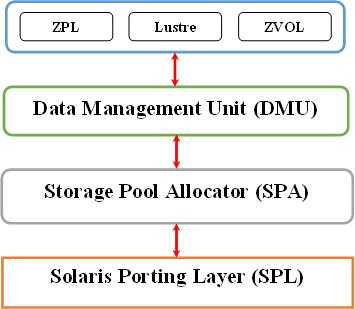
\includegraphics[width=8cm]{xx_klyga_arch_zfs}
  \caption{Архитектура ZFS для ОС Linux}
  \label{xx:klyga:fig1}
\end{figure}
\end{center}

Дополнительно был реализован еще один компонент IL включенный в состав ZFS в 2009 году ``Lustre'' позволяющий использовать ZFS в роли бэкенда для кластерных и сетевых файловых систем, например Lustre или pNFS (рисунок \ref{xx:klyga:fig2}).

\begin{center}
\begin{figure}[h!]
  \centering
  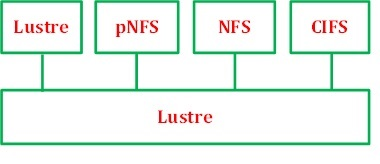
\includegraphics[width=8cm]{xx_klyga_zfs_lustre}
  \caption{Дополнительный компонент ``Lustre''}
  \label{xx:klyga:fig2}
\end{figure}
\end{center}

Использование данного компонента позволяет упростить интеграцию распределенных и сетевых файловых систем с ZFS, однако, при этом она остается локальной файловой системой.

\textbf{Возможности ZFS на базе проекта ``ZFS on Linux''}

Функциональные возможности ZFS на базе проекта “ZFS on Linux”:

\begin{itemize}
  \item режим multihost (MMP, Multi Modifier Protection);
  \item расширенная система квот;
  \item шифрование наборов данных;
  \item раздельный выбор классов распределения блоков (allocation classes);
  \item использование векторных процессорных инструкций для ускорения реализация RAIDZ и вычисления контрольных сумм;
  \item поддержку хранения контрольных сумм с использованием более надёжных криптографических хэшей SHA-512, Skein и Edon-R;
  \item защиту операций импорта пула в отказоусточивых конфигурациях;
  \item поддержка больших dnode для оптимизации работы с метаданными;
  \item дополнительные параметры (более 50) для тонкой настройки работы модуля ядра;
  \item улучшенный инструментарий командной строки.
\end{itemize}

Дополнительные возможности определяются версией модуля и ядра дистрибутива ОС Linux.

\subsection*{Дальнейшее развитие ZFS в рамках проекта \linebreak openZFS}

До конца 2017 года основной вклад в развитие ZFS вносил проект ``ZFS on Linux'' совместно с компанией  Delphix с использованием наработок основанных на оригинальном коде ZFS, импортированном из проекта OpenSolaris и расширенном улучшениями и исправлениями от сообщества Illumos.

Однако в 2018 году компания Delphix приняла решение о прекращении поддержки развития ZFS и переходе на использование кода проекта  ``ZFS on Linux'' \cite{bib8}, что привело к стагнации проекта Illumos.

В конце 2018 года о намерении перейти на проект ``ZFS on Linux'' объявила команда разработчиков FreeBSD \cite{bib9}. Таким образом вся активность по развитию и сопровождению проектов связанных с открытыми реализациями ZFS на базе проекта openZFS сократилась до одного ``ZFS on Linux''.

Новый релиз модуля ZFS для ядра Linux версии 0.8.0 был представлен 23 мая 2019 года, и включает в себя много изменений и дополнений \cite{bib10}. Однако, при этом необходимо учитывать, что реализация ZFS на базе проекта openZFS не обеспечивает полноценной совместимости с продуктами компании Oracle и развивается отдельно.

\begin{thebibliography}{9}
\bibitem{bib1} {ZFS in Wikipedia \url{https://ru.wikipedia.org/wiki/ZFS}}
\bibitem{bib2} {Модуль ядра FUSE \url{https://en.wikipedia.org/wiki/Filesystem_in_Userspace}}
\bibitem{bib3} {DKMS on GitHub \url{https://github.com/dell/dkms}}
\bibitem{bib4} {The ELRepo Blog. kABI-tracking kmod  \url{http://elrepoproject.blogspot.com/2016/02/kabi-tracking-kmod-packages.html}}
\bibitem{bib5} {ZFS on Linux \url{https://zfsonlinux.org/index.html}}
\bibitem{bib6} {Проект openZFS \url{http://open-zfs.org}}
\bibitem{bib7} {Dustin Kirkland. ZFS Licensing and Linux \url{http://blog.dustinkirkland.com/2016/02/zfs-licensing-and-linux.html}}
\bibitem{bib8} {Delphix Blog. Kickoff to The Future \url{https://www.delphix.com/blog/kickoff-future-eko-2018}}
\bibitem{bib9} {The future of ZFS in FreeBSD \url{https://lists.freebsd.org/pipermail/freebsd-current/2018-December/072422.html}}
\bibitem{bib10} {ZFS on Linux. Release zfs-0.8.0 \url{https://github.com/zfsonlinux/zfs/releases}}\end{thebibliography}
\end{document}
